\section{Prompt Engineering for Text-to-Image Generation}

\subsection{Generated Images}

\begin{figure}[h]
    \centering
    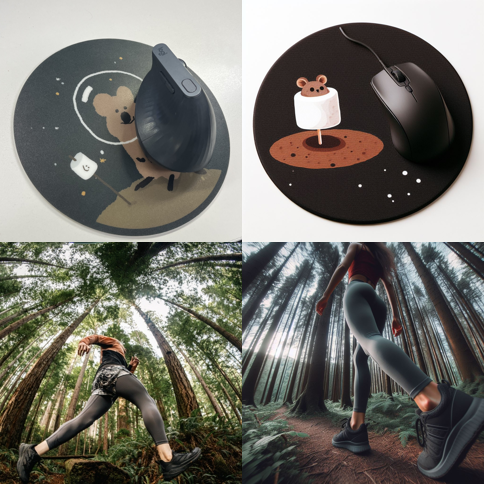
\includegraphics[width=0.5\textwidth]{imgs/p1_grid.png}
    \caption{Grid of images generated from prompts.}
    \label{fig:p1_grid}
\end{figure}

Fig.~\ref{fig:p1_grid} 와 같이 이미지를 생성하였다.
\texttt{image1\_given.png}와 \texttt{image1\_gen.png} 사이의 유사도는 0.6216 이고,
\texttt{image2\_given.png}와 \texttt{image2\_gen.png} 사이의 유사도는 0.6502 이다.

\subsection{Trials}

시도한 생성형 AI는 Stable Diffusion, wrtn(뤼튼, SDXL), DALL-E 3이다.
이 중 DALL-E 3가 가장 성능이 좋았다. 특히 \texttt{image1}에 있어 '흰 배경에 검은 마우스패드'를
정확히 이해하고 그림에 표현한 AI는 DALL-E 3가 유일했다.

또한, 생성된 이미지들은 사람이 보았을 때 전체적인 형태가 원본 이미지와 크게 닮지 않았다.
오히려 사람이 보았을 때 비슷한 형태라고 생각되는 이미지는 유사도가 낮게 나왔다.
